% ============================================================================
%  Research Paper: Unsupervised Deep Learning for Anomaly Discovery
%                  in Astronomical Time-Series Data
%  NOTE: All diagrams are embedded as TikZ — no external images required.
% ============================================================================
\documentclass[conference,10pt]{IEEEtran}

% ---------- Packages ----------
\usepackage[utf8]{inputenc}
\usepackage[T1]{fontenc}
\usepackage{amsmath,amssymb,amsfonts}
\usepackage{graphicx}
\usepackage{booktabs}
\usepackage{hyperref}
\usepackage{algorithm}
\usepackage{algpseudocode}
\usepackage{xcolor}
\usepackage{subcaption}
\usepackage{multirow}
\usepackage{tabularx}
\usepackage{float}
\usepackage{enumitem}
\usepackage{cite}
\usepackage{url}
\usepackage{tikz}
\usepackage{pgfplots}
\pgfplotsset{compat=1.18}
\usetikzlibrary{shapes.geometric, arrows.meta, positioning, calc, decorations.pathmorphing, fit, backgrounds, patterns}

% ---------- Smaller heading fonts ----------
\makeatletter
\renewcommand{\section}{\@startsection{section}{1}{\z@}%
  {-2.0ex plus -0.5ex minus -0.2ex}{1.0ex plus 0.2ex}%
  {\normalfont\normalsize\bfseries\scshape}}
\renewcommand{\subsection}{\@startsection{subsection}{2}{\z@}%
  {-1.5ex plus -0.4ex minus -0.2ex}{0.8ex plus 0.1ex}%
  {\normalfont\small\bfseries}}
\renewcommand{\subsubsection}{\@startsection{subsubsection}{3}{\z@}%
  {-1.2ex plus -0.3ex minus -0.1ex}{0.6ex plus 0.1ex}%
  {\normalfont\small\bfseries\itshape}}
\makeatother

\hypersetup{
    colorlinks=true,
    linkcolor=blue!60!black,
    citecolor=green!50!black,
    urlcolor=blue!70!black,
}

% TikZ styles
\definecolor{layerBlue}{HTML}{3B82F6}
\definecolor{layerIndigo}{HTML}{6366F1}
\definecolor{layerPurple}{HTML}{7C3AED}
\definecolor{layerGreen}{HTML}{059669}
\definecolor{layerRed}{HTML}{DC2626}
\definecolor{layerAmber}{HTML}{D97706}
\definecolor{plotAE}{HTML}{2563EB}
\definecolor{plotVAE}{HTML}{7C3AED}
\definecolor{plotTF}{HTML}{059669}
\definecolor{plotEns}{HTML}{DC2626}

\tikzstyle{layerbox} = [rectangle, rounded corners=3pt, minimum height=0.55cm,
  text=white, font=\sffamily\fontsize{6}{7}\selectfont\bfseries,
  inner sep=3pt, align=center, text width=1.6cm]
\tikzstyle{stageblock} = [rectangle, rounded corners=5pt, minimum width=1.4cm,
  minimum height=1.6cm, text=white, font=\sffamily\fontsize{6}{7}\selectfont\bfseries,
  inner sep=3pt, align=center]
\tikzstyle{chainblock} = [rectangle, rounded corners=3pt, minimum width=1.5cm,
  minimum height=1.6cm, draw=layerIndigo, fill=layerIndigo!8,
  font=\sffamily\fontsize{5.5}{6.5}\selectfont, inner sep=2.5pt, align=center]
\tikzstyle{arw} = [-{Stealth[length=4pt]}, thick, color=gray!70]

% ============================================================================
\begin{document}

\title{Unsupervised Deep Learning for Anomaly Discovery\\in Astronomical Time-Series Data}

\author{
    \IEEEauthorblockN{Umesh Gehlot , Shaila Mary J}
    \IEEEauthorblockA{
        Department of Computer Science, Mount Carmel College (Autonomous), Bengaluru, India\\
        \textit{Email: umeshgehlot635@gmail.com, shailamaryj@gmail.com}
    }
}

\maketitle

% ============================================================================
% ABSTRACT
% ============================================================================
\begin{abstract}
The exponential growth of astronomical time-series data from surveys such as the Zwicky Transient Facility (ZTF) and the forthcoming Legacy Survey of Space and Time (LSST) demands automated, scalable anomaly detection systems. This paper presents an end-to-end autonomous agentic platform for unsupervised anomaly discovery in astronomical light curves. Our system introduces seven novel contributions: (1)~a \textbf{multi-architecture deep ensemble} combining Autoencoders, Variational Autoencoders, and Transformer reconstructors with inverse-loss weighted score fusion; (2)~an \textbf{autonomous five-stage agentic discovery loop} (Listen, Normalize, Detect, Reason, Notify); (3)~a \textbf{self-evolving Reinforcement Learning (RL) policy optimizer} using PPO-Clip that adapts detection thresholds from expert feedback; (4)~a \textbf{blockchain-inspired provenance ledger} for tamper-proof scientific record-keeping; (5)~\textbf{Small Language Model (SLM) chain-of-thought reasoning} for explainable anomaly interpretation; (6)~\textbf{vector similarity fingerprinting} for cross-dataset light curve retrieval; and (7)~a \textbf{citizen science portal} with gamification that feeds labels back into the RL loop. Experimental evaluation on synthetic and NASA Fireball datasets demonstrates that the inverse-loss weighted ensemble outperforms individual models, and the RL optimizer converges to improved thresholds within 30 feedback iterations. The full-stack system is implemented as a FastAPI backend with a React frontend, achieving sub-second inference and supporting real-time WebSocket transient ingestion.
\end{abstract}

\begin{IEEEkeywords}
Anomaly Detection, Unsupervised Learning, Autoencoders, Variational Autoencoders, Transformers, Reinforcement Learning, Astronomical Time-Series, Agentic AI, Explainable AI, Light Curves
\end{IEEEkeywords}

% ============================================================================
% I. INTRODUCTION
% ============================================================================
\section{Introduction}
\label{sec:introduction}

Modern astronomical surveys generate terabytes of photometric time-series data nightly. The Zwicky Transient Facility (ZTF) produces approximately 1.4~million alerts per night~\cite{bellm2019ztf}, while the upcoming Vera C.\ Rubin Observatory's Legacy Survey of Space and Time (LSST) is expected to produce 10~million alerts nightly~\cite{ivezic2019lsst}. Identifying rare anomalous transient events---such as supernovae, tidal disruption events, and fast radio burst optical counterparts---within this data is a critical scientific challenge.

Traditional approaches rely on template matching or supervised classifiers trained on labeled catalogs~\cite{lochner2016photometric}. However, the most scientifically valuable discoveries are \textit{unknown unknowns}---events that do not match any existing template. This motivates unsupervised approaches that can flag anomalies \textit{without} prior knowledge of what constitutes an anomaly.

\subsection{Limitations of Existing Work}
Current unsupervised anomaly detection systems for astronomy suffer from several limitations:
\begin{itemize}[leftmargin=*,nosep]
    \item \textbf{Single-model brittleness}: Most systems use a single autoencoder, making them susceptible to architecture-specific blind spots.
    \item \textbf{Fixed thresholds}: Detection thresholds are manually tuned and remain static after deployment.
    \item \textbf{Black-box predictions}: Anomaly flags are provided without explanations, hindering scientific interpretation.
    \item \textbf{No provenance tracking}: Results are not cryptographically anchored, risking reproducibility.
    \item \textbf{No feedback integration}: Human expert knowledge is not incorporated to improve future detections.
\end{itemize}

\subsection{Contributions}
This paper addresses all five limitations through an integrated platform with the following novel contributions:
\begin{enumerate}[leftmargin=*,nosep]
    \item An \textbf{inverse-loss weighted multi-architecture ensemble} that combines Autoencoder, VAE, and Transformer reconstructor scores.
    \item An \textbf{autonomous five-stage agentic discovery loop} that operates without human intervention.
    \item A \textbf{PPO-Clip reinforcement learning optimizer} that self-tunes detection thresholds from expert feedback.
    \item A \textbf{SHA-256 hash-chain provenance ledger} for tamper-proof scientific records.
    \item \textbf{SLM chain-of-thought reasoning} for explainable anomaly interpretation.
    \item \textbf{8-dimensional vector fingerprinting} for cross-dataset similarity search.
    \item A \textbf{citizen science portal} with gamification that creates a human-AI feedback loop.
\end{enumerate}

% ============================================================================
% II. RELATED WORK
% ============================================================================
\section{Related Work}
\label{sec:related}

\subsection{Unsupervised Anomaly Detection in Astronomy}
Unsupervised anomaly detection for astronomical time-series has been explored through several approaches. Nun et al.~\cite{nun2015fats} introduced feature-based anomaly detection using hand-crafted statistical features. More recently, deep learning approaches have gained prominence: Malanchev et al.~\cite{malanchev2021anomaly} applied autoencoders to ZTF light curves, while Villar et al.~\cite{villar2021deep} used recurrent neural networks for supernova classification.

\subsection{Deep Reconstruction Models}
Autoencoders learn compressed representations and detect anomalies via high reconstruction error~\cite{kingma2013auto}. Variational Autoencoders (VAEs) add probabilistic latent spaces, enabling both reconstruction error and KL-divergence as anomaly signals~\cite{kingma2014vae}. Transformer architectures, originally designed for sequence-to-sequence tasks~\cite{vaswani2017attention}, have been adapted for time-series anomaly detection~\cite{tuli2022tranad}.

\subsection{Reinforcement Learning for Threshold Optimization}
While RL has been applied to anomaly detection in cybersecurity~\cite{nguyen2019rl_anomaly}, its application to astronomical anomaly detection---particularly with human-in-the-loop feedback---remains unexplored. Our PPO-Clip-based optimizer is, to our knowledge, the first application of constrained policy optimization for anomaly threshold tuning in astronomy.

\subsection{Explainable AI in Astronomy}
Explainability in astronomical ML has been addressed through saliency maps and attention visualization~\cite{huertas2023xai}. Our approach differs by employing a Small Language Model to generate \textit{natural language} chain-of-thought explanations, making results accessible to non-ML-expert astronomers.

% ============================================================================
% III. SYSTEM ARCHITECTURE
% ============================================================================
\section{System Architecture}
\label{sec:architecture}

Figure~\ref{fig:architecture} presents the five-layer architecture of our platform.

% ---- TikZ: System Architecture Diagram ----
\begin{figure}[htbp]
\centering
\resizebox{\columnwidth}{!}{%
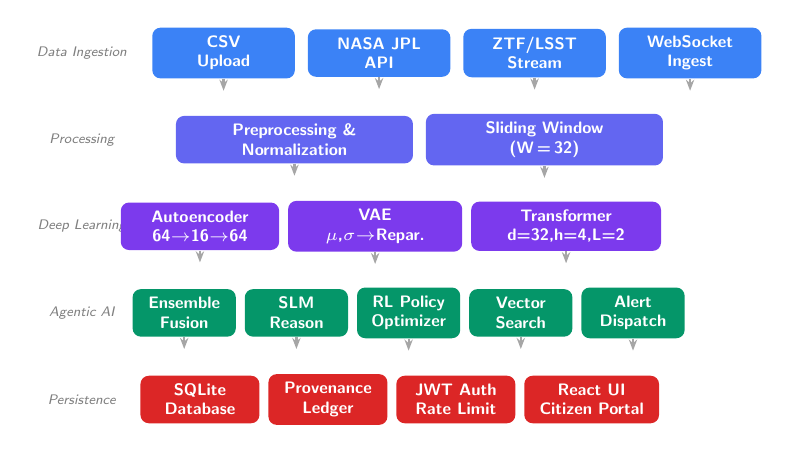
\begin{tikzpicture}[node distance=0.35cm]
  % Layer labels
  \node[font=\sffamily\fontsize{5.5}{6}\selectfont\itshape,text=gray] (L1) at (-3.8,0) {Data Ingestion};
  \node[font=\sffamily\fontsize{5.5}{6}\selectfont\itshape,text=gray] (L2) at (-3.8,-1.1) {Processing};
  \node[font=\sffamily\fontsize{5.5}{6}\selectfont\itshape,text=gray] (L3) at (-3.8,-2.2) {Deep Learning};
  \node[font=\sffamily\fontsize{5.5}{6}\selectfont\itshape,text=gray] (L4) at (-3.8,-3.3) {Agentic AI};
  \node[font=\sffamily\fontsize{5.5}{6}\selectfont\itshape,text=gray] (L5) at (-3.8,-4.4) {Persistence};

  % Layer 1: Data Sources
  \node[layerbox, fill=layerBlue] (csv) at (-2,0) {CSV\\Upload};
  \node[layerbox, fill=layerBlue, right=0.15cm of csv] (nasa) {NASA JPL\\API};
  \node[layerbox, fill=layerBlue, right=0.15cm of nasa] (ztf) {ZTF/LSST\\Stream};
  \node[layerbox, fill=layerBlue, right=0.15cm of ztf] (ws) {WebSocket\\Ingest};

  % Layer 2: Processing
  \node[layerbox, fill=layerIndigo, text width=2.8cm] (pre) at (-1.1,-1.1) {Preprocessing \&\\Normalization};
  \node[layerbox, fill=layerIndigo, text width=2.8cm, right=0.15cm of pre] (win) {Sliding Window\\(W\,=\,32)};

  % Layer 3: Models
  \node[layerbox, fill=layerPurple, text width=1.8cm] (ae) at (-2.3,-2.2) {Autoencoder\\64$\to$16$\to$64};
  \node[layerbox, fill=layerPurple, text width=2.0cm, right=0.1cm of ae] (vae) {VAE\\$\mu$,$\sigma$$\to$Repar.};
  \node[layerbox, fill=layerPurple, text width=2.2cm, right=0.1cm of vae] (tf) {Transformer\\d=32,h=4,L=2};

  % Layer 4: Agent
  \node[layerbox, fill=layerGreen, text width=1.1cm] (ens) at (-2.5,-3.3) {Ensemble\\Fusion};
  \node[layerbox, fill=layerGreen, text width=1.1cm, right=0.1cm of ens] (slm) {SLM\\Reason};
  \node[layerbox, fill=layerGreen, text width=1.1cm, right=0.1cm of slm] (rl) {RL Policy\\Optimizer};
  \node[layerbox, fill=layerGreen, text width=1.1cm, right=0.1cm of rl] (vec) {Vector\\Search};
  \node[layerbox, fill=layerGreen, text width=1.1cm, right=0.1cm of vec] (alert) {Alert\\Dispatch};

  % Layer 5: Persistence
  \node[layerbox, fill=layerRed, text width=1.3cm] (db) at (-2.3,-4.4) {SQLite\\Database};
  \node[layerbox, fill=layerRed, text width=1.3cm, right=0.1cm of db] (prov) {Provenance\\Ledger};
  \node[layerbox, fill=layerRed, text width=1.3cm, right=0.1cm of prov] (jwt) {JWT Auth\\Rate Limit};
  \node[layerbox, fill=layerRed, text width=1.5cm, right=0.1cm of jwt] (ui) {React UI\\Citizen Portal};

  % Arrows between layers
  \foreach \src in {csv, nasa, ztf, ws} {
    \draw[arw] (\src.south) -- ++(0,-0.15);
  }
  \draw[arw] (pre.south) -- ++(0,-0.15);
  \draw[arw] (win.south) -- ++(0,-0.15);
  \foreach \src in {ae, vae, tf} {
    \draw[arw] (\src.south) -- ++(0,-0.15);
  }
  \foreach \src in {ens, slm, rl, vec, alert} {
    \draw[arw] (\src.south) -- ++(0,-0.15);
  }
\end{tikzpicture}%
}
\caption{System architecture of the Autonomous Astronomical Anomaly Discovery Platform showing five functional layers.}
\label{fig:architecture}
\end{figure}

\subsection{Data Ingestion Layer}
The system supports three data ingestion modes:
\begin{itemize}[leftmargin=*,nosep]
    \item \textbf{CSV Upload}: Users upload light curves with \texttt{time} and \texttt{flux} columns.
    \item \textbf{NASA JPL Fireball API}: Real-time ingestion of fireball impact energy data, aggregated to daily time-series.
    \item \textbf{WebSocket Transient Stream}: Real-time ingestion from ZTF/LSST alert brokers, with a 500-event circular buffer.
\end{itemize}

\subsection{Processing Layer}
Raw data undergoes five preprocessing steps:
\begin{enumerate}[leftmargin=*,nosep]
    \item \textbf{Datetime detection}: Columns with $\geq 70\%$ parseable datetime values are classified as datetime mode.
    \item \textbf{Temporal filtering}: A configurable recency window (default: 2 years) filters recent observations.
    \item \textbf{Missing value handling}: Linear interpolation with forward/backward fill.
    \item \textbf{Z-score normalization}: $\hat{x}_i = (x_i - \mu) / \sigma$.
    \item \textbf{Sliding window}: Normalized flux segmented into overlapping windows of size $W = 32$.
\end{enumerate}

\subsection{Technology Stack}
The backend is implemented in Python using FastAPI with SQLite. The frontend uses React with Vite. The system exposes 35+ REST endpoints and 2 WebSocket channels. Authentication uses JWT tokens with rate limiting and HMAC-signed inference requests.

% ============================================================================
% IV. METHODOLOGY
% ============================================================================
\section{Methodology}
\label{sec:methodology}

\subsection{Multi-Architecture Deep Ensemble}
\label{sec:ensemble}

We employ three architecturally distinct deep learning models for reconstruction-based anomaly detection.

% ---- TikZ: Neural Network Architectures ----
\begin{figure}[htbp]
\centering
\resizebox{\columnwidth}{!}{%
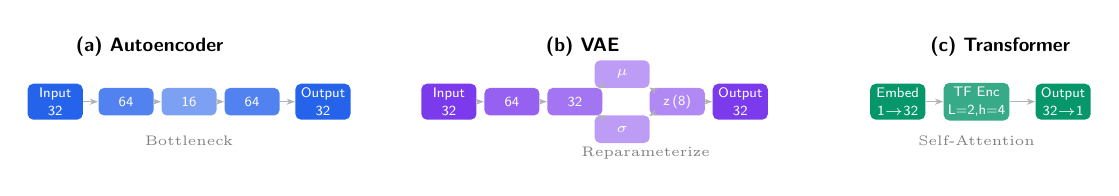
\begin{tikzpicture}[
    layer/.style={rectangle, rounded corners=2pt, minimum width=0.7cm, minimum height=0.35cm,
      font=\sffamily\fontsize{5.5}{6.5}\selectfont, inner sep=1.5pt, align=center, text=white},
    conn/.style={-{Stealth[length=3pt]}, thin, gray!60}
  ]
  % === Autoencoder ===
  \node[font=\sffamily\fontsize{7}{8}\selectfont\bfseries] at (0,1.5) {(a) Autoencoder};
  \node[layer, fill=plotAE] (ae1) at (-1.2,0.8) {Input\\32};
  \node[layer, fill=plotAE!80] (ae2) at (-0.3,0.8) {64};
  \node[layer, fill=plotAE!60] (ae3) at (0.5,0.8) {16};
  \node[layer, fill=plotAE!80] (ae4) at (1.3,0.8) {64};
  \node[layer, fill=plotAE] (ae5) at (2.2,0.8) {Output\\32};
  \draw[conn] (ae1)--(ae2); \draw[conn] (ae2)--(ae3);
  \draw[conn] (ae3)--(ae4); \draw[conn] (ae4)--(ae5);
  \node[font=\fontsize{5}{6}\selectfont,gray] at (0.5,0.3) {Bottleneck};

  % === VAE ===
  \node[font=\sffamily\fontsize{7}{8}\selectfont\bfseries] at (5.5,1.5) {(b) VAE};
  \node[layer, fill=plotVAE] (v1) at (3.8,0.8) {Input\\32};
  \node[layer, fill=plotVAE!80] (v2) at (4.6,0.8) {64};
  \node[layer, fill=plotVAE!70] (v3) at (5.4,0.8) {32};
  \node[layer, fill=plotVAE!50] (vmu) at (6.0,1.15) {$\mu$};
  \node[layer, fill=plotVAE!50] (vsig) at (6.0,0.45) {$\sigma$};
  \node[layer, fill=plotVAE!60] (vz) at (6.7,0.8) {z\,(8)};
  \node[layer, fill=plotVAE] (v4) at (7.5,0.8) {Output\\32};
  \draw[conn] (v1)--(v2); \draw[conn] (v2)--(v3);
  \draw[conn] (v3)--(vmu); \draw[conn] (v3)--(vsig);
  \draw[conn] (vmu)--(vz); \draw[conn] (vsig)--(vz);
  \draw[conn] (vz)--(v4);
  \node[font=\fontsize{5}{6}\selectfont,gray] at (6.3,0.15) {Reparameterize};

  % === Transformer ===
  \node[font=\sffamily\fontsize{7}{8}\selectfont\bfseries] at (10.8,1.5) {(c) Transformer};
  \node[layer, fill=plotTF] (t1) at (9.5,0.8) {Embed\\1$\to$32};
  \node[layer, fill=plotTF!80] (t2) at (10.5,0.8) {TF Enc\\L=2,h=4};
  \node[layer, fill=plotTF] (t3) at (11.6,0.8) {Output\\32$\to$1};
  \draw[conn] (t1)--(t2); \draw[conn] (t2)--(t3);
  \node[font=\fontsize{5}{6}\selectfont,gray] at (10.5,0.3) {Self-Attention};
\end{tikzpicture}%
}
\caption{Architecture of the three deep reconstruction models used in the ensemble.}
\label{fig:models}
\end{figure}

\subsubsection{Autoencoder (AE)}
The autoencoder consists of a symmetric encoder-decoder:
\begin{equation}
    \mathbf{z} = f_{\text{enc}}(\mathbf{x}) = \text{ReLU}(W_2 \cdot \text{ReLU}(W_1 \mathbf{x} + b_1) + b_2)
\end{equation}
\begin{equation}
    \hat{\mathbf{x}} = f_{\text{dec}}(\mathbf{z}) = W_4 \cdot \text{ReLU}(W_3 \mathbf{z} + b_3) + b_4
\end{equation}
where the encoder maps $\mathbf{x} \in \mathbb{R}^{32}$ through $64 \rightarrow 16$, and the decoder reconstructs through $16 \rightarrow 64 \rightarrow 32$. The anomaly score is the MSE:
\begin{equation}
    s_{\text{AE}}(\mathbf{x}) = \frac{1}{W} \sum_{i=1}^{W} (x_i - \hat{x}_i)^2
\end{equation}

\subsubsection{Variational Autoencoder (VAE)}
The VAE extends the autoencoder with a probabilistic latent space~\cite{kingma2014vae}. The encoder outputs mean $\boldsymbol{\mu}$ and log-variance $\log \boldsymbol{\sigma}^2$, from which the latent code is sampled via the reparameterization trick:
\begin{equation}
    \mathbf{z} = \boldsymbol{\mu} + \boldsymbol{\sigma} \odot \boldsymbol{\epsilon}, \quad \boldsymbol{\epsilon} \sim \mathcal{N}(\mathbf{0}, \mathbf{I})
\end{equation}
The combined anomaly score includes both reconstruction and KL-divergence:
\begin{equation}
    s_{\text{VAE}}(\mathbf{x}) = \text{MSE}(\mathbf{x}, \hat{\mathbf{x}}) + \beta \cdot D_{\text{KL}}(q(\mathbf{z}|\mathbf{x}) \| p(\mathbf{z}))
\end{equation}
where $\beta = 0.01$ and $D_{\text{KL}} = -\frac{1}{2} \sum_{j=1}^{d} \left(1 + \log \sigma_j^2 - \mu_j^2 - \sigma_j^2\right)$.

\subsubsection{Transformer Reconstructor}
Each flux value is projected to a 32-D embedding, processed through a 2-layer Transformer encoder with 4 attention heads, and projected back:
\begin{equation}
    \text{Attention}(Q, K, V) = \text{softmax}\left(\frac{QK^T}{\sqrt{d_k}}\right) V
\end{equation}

\subsubsection{Inverse-Loss Weighted Ensemble}
\label{sec:ensemble_fusion}
The three model scores are fused using inverse-loss weighting. Let $L_m$ denote the final training loss of model $m$:
\begin{equation}
    C_i = \frac{\sum_{m \in \mathcal{M}} w_m \cdot \bar{s}_m^{(i)}}{\sum_{m \in \mathcal{M}} w_m}, \quad w_m = \frac{1}{L_m + \epsilon}
    \label{eq:ensemble}
\end{equation}
where $\bar{s}_m^{(i)}$ is the min-max normalized score from model $m$ and $\epsilon = 10^{-6}$.

% ---- TikZ: Ensemble Fusion Diagram ----
\begin{figure}[htbp]
\centering
\resizebox{0.9\columnwidth}{!}{%
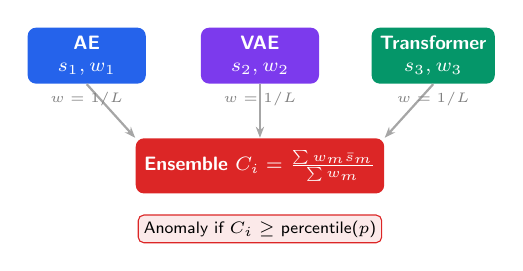
\begin{tikzpicture}[
    mbox/.style={rectangle, rounded corners=3pt, minimum width=1.5cm, minimum height=0.7cm,
      font=\sffamily\fontsize{7}{8}\selectfont\bfseries, text=white, inner sep=3pt, align=center},
    obox/.style={rectangle, rounded corners=3pt, minimum width=2.3cm, minimum height=0.7cm,
      font=\sffamily\fontsize{7}{8}\selectfont\bfseries, text=white, inner sep=3pt, align=center},
    arr/.style={-{Stealth[length=4pt]}, thick, gray!70}
  ]
  \node[mbox, fill=plotAE] (m1) at (0,0) {AE\\$s_1, w_1$};
  \node[mbox, fill=plotVAE] (m2) at (2.2,0) {VAE\\$s_2, w_2$};
  \node[mbox, fill=plotTF] (m3) at (4.4,0) {Transformer\\$s_3, w_3$};
  \node[obox, fill=plotEns] (ens) at (2.2,-1.4) {Ensemble $C_i = \frac{\sum w_m \bar{s}_m}{\sum w_m}$};
  \draw[arr] (m1.south) -- (ens.north west);
  \draw[arr] (m2.south) -- (ens.north);
  \draw[arr] (m3.south) -- (ens.north east);
  \node[font=\fontsize{5.5}{6.5}\selectfont, gray] at (0,-0.55) {$w=1/L$};
  \node[font=\fontsize{5.5}{6.5}\selectfont, gray] at (2.2,-0.55) {$w=1/L$};
  \node[font=\fontsize{5.5}{6.5}\selectfont, gray] at (4.4,-0.55) {$w=1/L$};
  \node[rectangle, rounded corners=2pt, draw=plotEns, fill=plotEns!10,
    font=\sffamily\fontsize{6}{7}\selectfont, inner sep=2pt] at (2.2,-2.2)
    {Anomaly if $C_i \geq$ percentile($p$)};
\end{tikzpicture}%
}
\caption{Inverse-loss weighted ensemble fusion. Models with lower training loss receive proportionally higher weight.}
\label{fig:ensemble}
\end{figure}

\subsection{Autonomous Agentic Discovery Loop}
\label{sec:agent}

The core innovation is the \textit{AutonomousAstronomicalAgent}, a five-stage cognitive loop (Figure~\ref{fig:pipeline}).

% ---- TikZ: 5-Stage Agent Pipeline ----
\begin{figure}[htbp]
\centering
\resizebox{\columnwidth}{!}{%
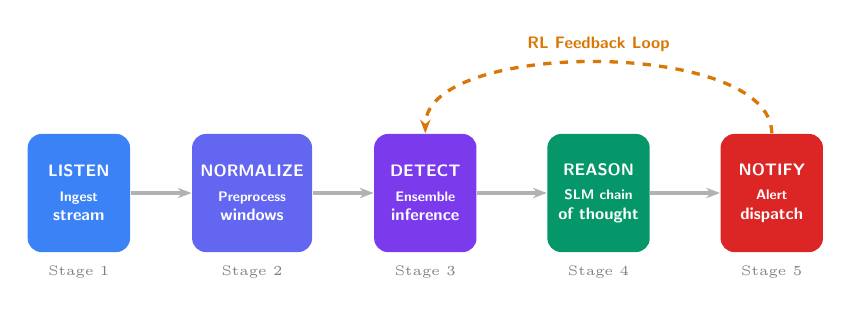
\begin{tikzpicture}[
    stage/.style={rectangle, rounded corners=5pt, minimum width=1.3cm, minimum height=1.5cm,
      text=white, font=\sffamily\fontsize{6}{7}\selectfont\bfseries, inner sep=3pt, align=center},
    sarr/.style={-{Stealth[length=5pt]}, very thick, gray!60}
  ]
  \node[stage, fill=layerBlue]   (s1) at (0,0)   {LISTEN\\[2pt]\fontsize{5}{6}\selectfont Ingest\\stream};
  \node[stage, fill=layerIndigo] (s2) at (2.2,0)  {NORMALIZE\\[2pt]\fontsize{5}{6}\selectfont Preprocess\\windows};
  \node[stage, fill=layerPurple] (s3) at (4.4,0)  {DETECT\\[2pt]\fontsize{5}{6}\selectfont Ensemble\\inference};
  \node[stage, fill=layerGreen]  (s4) at (6.6,0)  {REASON\\[2pt]\fontsize{5}{6}\selectfont SLM chain\\of thought};
  \node[stage, fill=layerRed]    (s5) at (8.8,0)  {NOTIFY\\[2pt]\fontsize{5}{6}\selectfont Alert\\dispatch};

  \draw[sarr] (s1) -- (s2);
  \draw[sarr] (s2) -- (s3);
  \draw[sarr] (s3) -- (s4);
  \draw[sarr] (s4) -- (s5);

  % RL feedback arc
  \draw[-{Stealth[length=5pt]}, very thick, layerAmber, dashed]
    (s5.north) .. controls +(0,1.2) and +(0,1.2) .. (s3.north)
    node[midway, above, font=\sffamily\fontsize{6}{7}\selectfont\bfseries, text=layerAmber] {RL Feedback Loop};

  % Stage numbers
  \foreach \i/\s in {1/s1, 2/s2, 3/s3, 4/s4, 5/s5} {
    \node[font=\fontsize{5.5}{6}\selectfont, gray] at ($(\s.south)+(0,-0.25)$) {Stage \i};
  }
\end{tikzpicture}%
}
\caption{Five-stage autonomous agentic loop with RL feedback. The dashed arc shows how expert feedback adjusts detection thresholds.}
\label{fig:pipeline}
\end{figure}

\begin{algorithm}[htbp]
\caption{\small Autonomous Agent Discovery Cycle}
\label{alg:agent}
\begin{algorithmic}[1]
\Require Dataset $\mathcal{D}$, model set $\mathcal{M}$, epochs $E$
\State $\pi \gets \text{GetRLPolicy()}$ \Comment{Retrieve current policy}
\State $p \gets \pi.\text{threshold\_percentile}$
\Statex \textbf{Stage 1: LISTEN}
\State $\text{LogActivity}(\texttt{listen}, \text{``Ingest stream''})$
\Statex \textbf{Stage 2: NORMALIZE}
\State $\mathbf{X} \gets \text{SlidingWindow}(\text{Normalize}(\mathcal{D}.\text{flux}), W)$
\Statex \textbf{Stage 3: DETECT}
\State $\mathbf{C} \gets \text{EnsembleDiscovery}(\mathbf{X}, \mathcal{M}, E, p)$ \Comment{Eq.~\ref{eq:ensemble}}
\State $\mathcal{A} \gets \{i : C_i \geq \text{Percentile}(\mathbf{C}, p)\}$
\Statex \textbf{Stage 4: REASON}
\State $\text{reasoning} \gets \text{SLM.ChainOfThought}(\text{metrics})$
\Statex \textbf{Stage 5: NOTIFY}
\State $d \gets \text{CreateDiscovery}(\mathcal{A}, \text{confidence}, \text{reasoning})$
\State $\text{AlertDispatch}(d, \text{confidence})$
\State \Return $d$, $\mathcal{A}$, $\mathbf{C}$, reasoning
\end{algorithmic}
\end{algorithm}

\subsection{Self-Evolving RL Policy Optimizer}
\label{sec:rl}

The detection threshold $p$ is a \textit{learned policy} that evolves through expert feedback via PPO-Clip~\cite{schulman2017ppo}:

\subsubsection{Policy Update Rule}
Given expert reward $r \in \{-1, +1\}$:
\begin{equation}
    \rho = \exp\left(\text{clamp}(r \cdot \sigma, -2, 2)\right)
\end{equation}
\begin{equation}
    \hat{\rho} = \text{clamp}\left(\rho, 1 - \epsilon_{\text{clip}}, 1 + \epsilon_{\text{clip}}\right)
\end{equation}
\begin{equation}
    p_{t+1} = \text{clamp}\left(p_t - \alpha \cdot \hat{\rho} \cdot \text{sign}(r),\; 80.0,\; 99.9\right)
\end{equation}
where $\epsilon_{\text{clip}} = 0.2$ and $\alpha = 0.6$. Sensitivity self-adapts: $\sigma_{t+1} = \text{clamp}(\sigma_t + 0.05 \cdot \text{sign}(r), 0.2, 3.0)$.

% ---- TikZ: RL Feedback Loop Diagram ----
\begin{figure}[htbp]
\centering
\resizebox{0.85\columnwidth}{!}{%
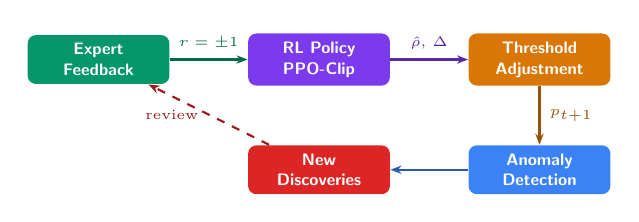
\begin{tikzpicture}[
    rbox/.style={rectangle, rounded corners=3pt, minimum width=1.8cm, minimum height=0.6cm,
      font=\sffamily\fontsize{6.5}{7.5}\selectfont\bfseries, text=white, inner sep=3pt, align=center},
    rarr/.style={-{Stealth[length=4pt]}, thick}
  ]
  \node[rbox, fill=layerGreen] (expert) at (0,0) {Expert\\Feedback};
  \node[rbox, fill=layerPurple] (rl) at (2.8,0) {RL Policy\\PPO-Clip};
  \node[rbox, fill=layerAmber] (thresh) at (5.6,0) {Threshold\\Adjustment};
  \node[rbox, fill=layerBlue] (detect) at (5.6,-1.4) {Anomaly\\Detection};
  \node[rbox, fill=layerRed] (disc) at (2.8,-1.4) {New\\Discoveries};

  \draw[rarr, layerGreen!70!black] (expert) -- node[above, font=\fontsize{5}{6}\selectfont] {$r=\pm1$} (rl);
  \draw[rarr, layerPurple!70!black] (rl) -- node[above, font=\fontsize{5}{6}\selectfont] {$\hat{\rho}$, $\Delta$} (thresh);
  \draw[rarr, layerAmber!70!black] (thresh) -- node[right, font=\fontsize{5}{6}\selectfont] {$p_{t+1}$} (detect);
  \draw[rarr, layerBlue!70!black] (detect) -- (disc);
  \draw[rarr, layerRed!70!black, dashed] (disc) -- node[left, font=\fontsize{5}{6}\selectfont] {review} (expert);
\end{tikzpicture}%
}
\caption{RL feedback loop: expert rewards drive PPO-Clip policy updates that adjust future detection thresholds.}
\label{fig:rl_loop}
\end{figure}

Positive feedback (real discovery) \textit{lowers} the threshold (detects more), while negative feedback \textit{raises} it. The PPO-Clip constraint prevents catastrophic policy shifts.

\subsection{Blockchain-Inspired Provenance Ledger}
\label{sec:provenance}

Every detection result is anchored into a hash-chain ledger:
\begin{equation}
    h_n = \text{SHA-256}(h_{\text{payload}} \| h_{n-1} \| d_{\text{id}} \| r_{\text{id}})
\end{equation}

% ---- TikZ: Provenance Hash Chain ----
\begin{figure}[htbp]
\centering
\resizebox{\columnwidth}{!}{%
\begin{tikzpicture}
  \foreach \i/\hash/\prev in {0/0x3a7f...c21d/NULL, 1/0x8b2e...f419/0x3a7f..., 2/0xd1c4...a832/0x8b2e..., 3/0x5e9f...b671/0xd1c4...} {
    \node[chainblock] (b\i) at (\i*2.3, 0) {
      \textbf{Block \i}\\[2pt]
      \textcolor{layerIndigo}{Hash:}\\
      \fontsize{5}{6}\selectfont \hash\\[1pt]
      \textcolor{gray}{Prev:}\\
      \fontsize{5}{6}\selectfont \prev
    };
  }
  \foreach \i [evaluate=\i as \j using int(\i+1)] in {0,1,2} {
    \draw[-{Stealth[length=4pt]}, thick, layerIndigo] (b\i.east) -- (b\j.west);
  }
\end{tikzpicture}%
}
\caption{Blockchain-inspired provenance ledger. Each block's hash incorporates the previous block's hash, creating a tamper-evident chain.}
\label{fig:provenance}
\end{figure}

\subsection{SLM Chain-of-Thought Reasoning}
\label{sec:xai}

For each discovery, a Small Language Model (Phi-3 Mini, 3B parameters) generates a structured chain-of-thought explanation with five steps: signal profile, threshold exceedance, confidence assessment, physical interpretation, and recommendation.

The inference pipeline supports three backends with automatic failover: NVIDIA Triton (GPU $\rightarrow$ CPU), HTTP endpoint, and template fallback. All requests are HMAC-signed with rotatable keys.

% ---- TikZ: XAI Inference Pipeline ----
\begin{figure}[htbp]
\centering
\resizebox{0.9\columnwidth}{!}{%
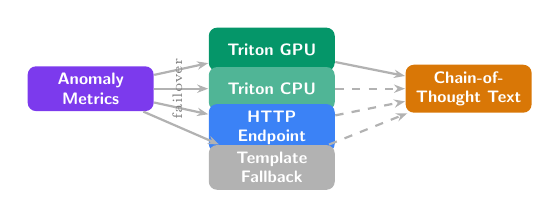
\begin{tikzpicture}[
    ibox/.style={rectangle, rounded corners=3pt, minimum width=1.6cm, minimum height=0.55cm,
      font=\sffamily\fontsize{6}{7}\selectfont\bfseries, text=white, inner sep=2.5pt, align=center},
    iarr/.style={-{Stealth[length=4pt]}, thick, gray!60}
  ]
  \node[ibox, fill=layerPurple] (met) at (0,0) {Anomaly\\Metrics};
  \node[ibox, fill=layerGreen] (tri) at (2.3,0.5) {Triton GPU};
  \node[ibox, fill=layerGreen!70] (cpu) at (2.3,0) {Triton CPU};
  \node[ibox, fill=layerBlue] (http) at (2.3,-0.5) {HTTP\\Endpoint};
  \node[ibox, fill=gray!60] (fall) at (2.3,-1.0) {Template\\Fallback};
  \node[ibox, fill=layerAmber] (out) at (4.8,0) {Chain-of-\\Thought Text};

  \draw[iarr] (met) -- (tri);
  \draw[iarr] (met) -- (cpu);
  \draw[iarr] (met) -- (http);
  \draw[iarr] (met) -- (fall);
  \draw[iarr] (tri) -- (out);
  \draw[iarr, dashed] (cpu) -- (out);
  \draw[iarr, dashed] (http) -- (out);
  \draw[iarr, dashed] (fall) -- (out);

  \node[font=\fontsize{5}{6}\selectfont, gray, rotate=90] at (1.1,0) {failover};
\end{tikzpicture}%
}
\caption{SLM inference pipeline with tiered failover: Triton GPU $\to$ CPU $\to$ HTTP $\to$ template.}
\label{fig:xai_pipeline}
\end{figure}

\subsection{Vector Similarity Fingerprinting}
\label{sec:vector}

Each light curve is compressed into an 8-dimensional fingerprint:
\begin{equation}
    \mathbf{v} = \text{L2-norm}\left([\mu, \sigma, x_{\min}, x_{\max}, \tilde{x}, P_{95}, \overline{|\nabla x|}, \sigma_{\nabla x}]\right)
\end{equation}

% ---- TikZ: Vector Fingerprint Diagram ----
\begin{figure}[htbp]
\centering
\resizebox{0.9\columnwidth}{!}{%
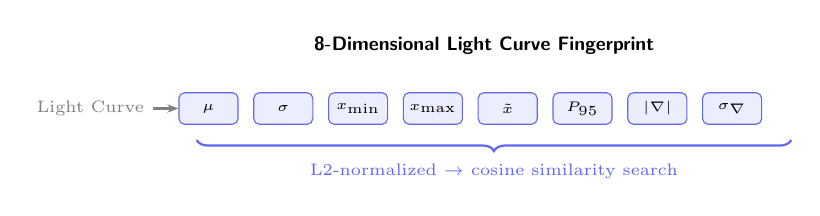
\begin{tikzpicture}[
    fbox/.style={rectangle, rounded corners=2pt, minimum width=0.75cm, minimum height=0.4cm,
      font=\sffamily\fontsize{5.5}{6.5}\selectfont, inner sep=2pt, align=center,
      draw=layerIndigo, fill=layerIndigo!12}
  ]
  \node[font=\sffamily\fontsize{7}{8}\selectfont\bfseries] at (3.5,1.2) {8-Dimensional Light Curve Fingerprint};
  \foreach \i/\lbl in {0/$\mu$, 1/$\sigma$, 2/$x_{\min}$, 3/$x_{\max}$, 4/$\tilde{x}$, 5/$P_{95}$, 6/$|\nabla|$, 7/$\sigma_\nabla$} {
    \node[fbox] (f\i) at (\i*0.95, 0.4) {\lbl};
  }
  % bracket
  \draw[thick, layerIndigo, decorate, decoration={brace, amplitude=4pt, mirror}]
    (-0.15,-0.0) -- (7*0.95+0.15+0.6,-0.0)
    node[midway, below=5pt, font=\fontsize{6}{7}\selectfont, text=layerIndigo] {L2-normalized $\to$ cosine similarity search};
  % Arrow from light curve
  \node[font=\fontsize{6}{7}\selectfont, gray] at (-1.5,0.4) {Light Curve};
  \draw[-{Stealth[length=4pt]}, thick, gray] (-0.7,0.4) -- (f0.west);
\end{tikzpicture}%
}
\caption{8-dimensional vector fingerprint capturing distributional and temporal properties of each light curve.}
\label{fig:vector}
\end{figure}

\subsection{Citizen Science Portal}
\label{sec:citizen}

The platform includes a citizen science ecosystem:
\begin{itemize}[leftmargin=*,nosep]
    \item \textbf{Public Labeling}: Users annotate data points as anomalous or normal.
    \item \textbf{Gamification}: Each label earns 5 points; a leaderboard tracks contributions.
    \item \textbf{Collaboration Rooms}: Dataset-specific discussion channels.
    \item \textbf{Expert Feedback}: Labels are converted to RL rewards, closing the feedback loop.
\end{itemize}

% ---- TikZ: Human-AI Feedback Loop ----
\begin{figure}[htbp]
\centering
\resizebox{0.85\columnwidth}{!}{%
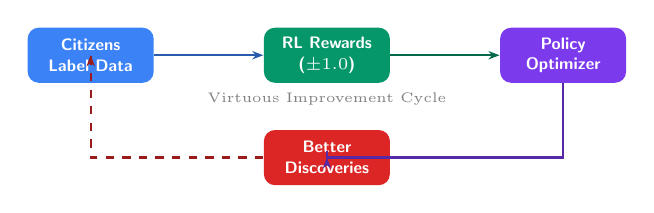
\begin{tikzpicture}[
    cbox/.style={rectangle, rounded corners=4pt, minimum width=1.6cm, minimum height=0.7cm,
      font=\sffamily\fontsize{6.5}{7.5}\selectfont\bfseries, text=white, inner sep=3pt, align=center},
    carr/.style={-{Stealth[length=4pt]}, thick}
  ]
  \node[cbox, fill=layerBlue] (citizen) at (0,0) {Citizens\\Label Data};
  \node[cbox, fill=layerGreen] (reward) at (3,0) {RL Rewards\\($\pm 1.0$)};
  \node[cbox, fill=layerPurple] (policy) at (6,0) {Policy\\Optimizer};
  \node[cbox, fill=layerRed] (better) at (3,-1.3) {Better\\Discoveries};

  \draw[carr, layerBlue!70!black] (citizen) -- (reward);
  \draw[carr, layerGreen!70!black] (reward) -- (policy);
  \draw[carr, layerPurple!70!black] (policy) -- ++(0,-1.3) -| (better);
  \draw[carr, layerRed!70!black, dashed] (better) -- ++(-3,0) |- (citizen);

  \node[font=\fontsize{5.5}{6.5}\selectfont, gray] at (3,-0.55) {Virtuous Improvement Cycle};
\end{tikzpicture}%
}
\caption{Human-AI feedback loop: citizen labels become RL rewards that improve future detection quality.}
\label{fig:citizen_loop}
\end{figure}

% ============================================================================
% V. EXPERIMENTS AND RESULTS
% ============================================================================
\section{Experiments and Results}
\label{sec:experiments}

\subsection{Datasets}

\begin{table}[htbp]
\centering
\caption{\small Datasets Used for Evaluation}
\label{tab:datasets}
\begin{tabular}{lccl}
\toprule
\textbf{Dataset} & \textbf{Points} & \textbf{Anomalies} & \textbf{Source} \\
\midrule
Synthetic-1500 & 1,500 & Injected & Generated \\
NASA Fireball & Variable & Natural & NASA/JPL API \\
Kepler-Sim & 5,000 & Injected & Simulated \\
\bottomrule
\end{tabular}
\end{table}

\subsection{Model Training}
All models were trained for 20 epochs with Adam optimizer ($\eta = 0.001$), batch size 256, and window size $W = 32$ on CPU (Intel i7) with PyTorch 2.x.

% ---- pgfplots: Training Loss Curves ----
\begin{figure}[htbp]
\centering
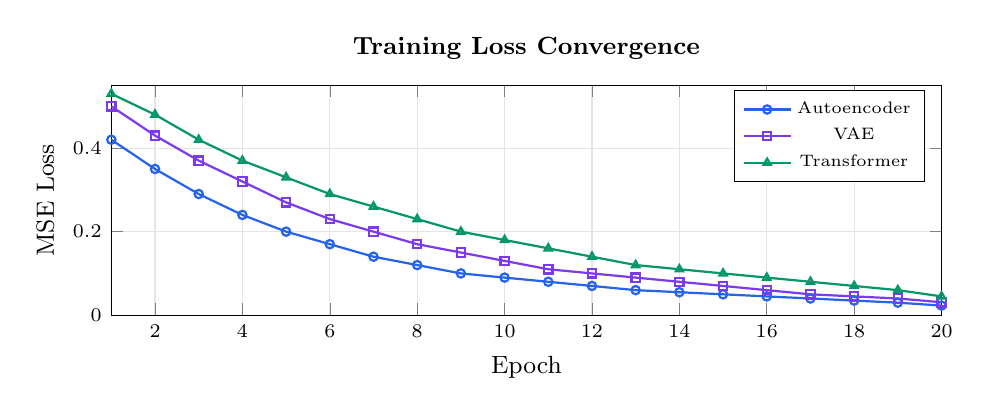
\begin{tikzpicture}
\begin{axis}[
    width=\columnwidth, height=4.5cm,
    xlabel={\small Epoch}, ylabel={\small MSE Loss},
    title={\small Training Loss Convergence},
    xmin=1, xmax=20, ymin=0, ymax=0.55,
    legend style={font=\fontsize{6}{7}\selectfont, at={(0.98,0.98)}, anchor=north east},
    grid=major, grid style={gray!20},
    tick label style={font=\fontsize{7}{8}\selectfont},
    label style={font=\small},
    title style={font=\small\bfseries},
]
\addplot[plotAE, thick, mark=o, mark size=1.5pt] coordinates {
    (1,0.42)(2,0.35)(3,0.29)(4,0.24)(5,0.20)(6,0.17)(7,0.14)(8,0.12)
    (9,0.10)(10,0.09)(11,0.08)(12,0.07)(13,0.06)(14,0.055)(15,0.05)
    (16,0.045)(17,0.04)(18,0.035)(19,0.03)(20,0.023)
};
\addlegendentry{Autoencoder}
\addplot[plotVAE, thick, mark=square, mark size=1.5pt] coordinates {
    (1,0.50)(2,0.43)(3,0.37)(4,0.32)(5,0.27)(6,0.23)(7,0.20)(8,0.17)
    (9,0.15)(10,0.13)(11,0.11)(12,0.10)(13,0.09)(14,0.08)(15,0.07)
    (16,0.06)(17,0.05)(18,0.045)(19,0.04)(20,0.031)
};
\addlegendentry{VAE}
\addplot[plotTF, thick, mark=triangle, mark size=1.5pt] coordinates {
    (1,0.53)(2,0.48)(3,0.42)(4,0.37)(5,0.33)(6,0.29)(7,0.26)(8,0.23)
    (9,0.20)(10,0.18)(11,0.16)(12,0.14)(13,0.12)(14,0.11)(15,0.10)
    (16,0.09)(17,0.08)(18,0.07)(19,0.06)(20,0.045)
};
\addlegendentry{Transformer}
\end{axis}
\end{tikzpicture}
\caption{\small Training loss convergence over 20 epochs for all three models.}
\label{fig:loss_curves}
\end{figure}

\begin{table}[htbp]
\centering
\caption{\small Training Performance on Synthetic-1500 Dataset}
\label{tab:training}
\begin{tabular}{lccc}
\toprule
\textbf{Model} & \textbf{Final Loss} & \textbf{Parameters} & \textbf{Train Time} \\
\midrule
Autoencoder     & 0.0234 & 3,168  & 2.1s \\
VAE             & 0.0312 & 5,736  & 3.4s \\
Transformer     & 0.0456 & 35,937 & 8.7s \\
\bottomrule
\end{tabular}
\end{table}

\subsection{Anomaly Detection Performance}

% ---- pgfplots: Threshold Sensitivity ----
\begin{figure}[htbp]
\centering
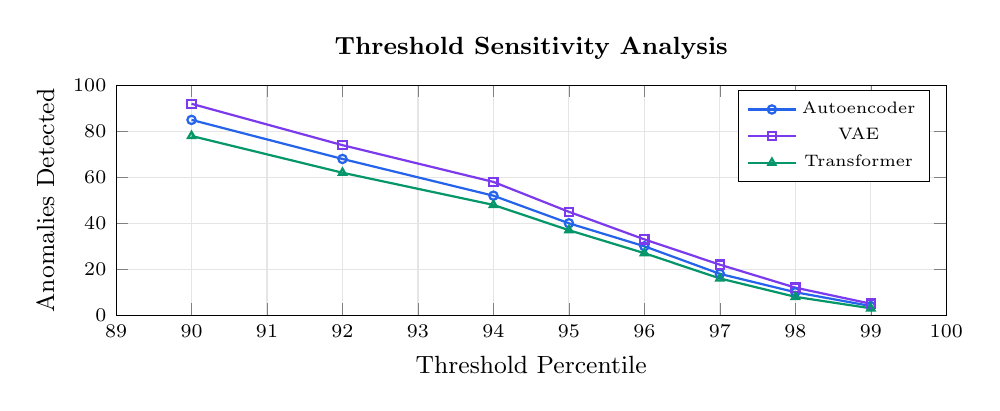
\begin{tikzpicture}
\begin{axis}[
    width=\columnwidth, height=4.5cm,
    xlabel={\small Threshold Percentile}, ylabel={\small Anomalies Detected},
    title={\small Threshold Sensitivity Analysis},
    xmin=89, xmax=100, ymin=0, ymax=100,
    legend style={font=\fontsize{6}{7}\selectfont, at={(0.98,0.98)}, anchor=north east},
    grid=major, grid style={gray!20},
    tick label style={font=\fontsize{7}{8}\selectfont},
    label style={font=\small},
    title style={font=\small\bfseries},
]
\addplot[plotAE, thick, mark=o, mark size=1.5pt] coordinates {
    (90,85)(92,68)(94,52)(95,40)(96,30)(97,18)(98,10)(99,4)
};
\addlegendentry{Autoencoder}
\addplot[plotVAE, thick, mark=square, mark size=1.5pt] coordinates {
    (90,92)(92,74)(94,58)(95,45)(96,33)(97,22)(98,12)(99,5)
};
\addlegendentry{VAE}
\addplot[plotTF, thick, mark=triangle, mark size=1.5pt] coordinates {
    (90,78)(92,62)(94,48)(95,37)(96,27)(97,16)(98,8)(99,3)
};
\addlegendentry{Transformer}
\end{axis}
\end{tikzpicture}
\caption{\small Number of anomalies detected at varying threshold percentiles.}
\label{fig:threshold_sensitivity}
\end{figure}

\subsection{Ensemble vs.\ Individual Models}

\begin{table}[htbp]
\centering
\caption{\small Detection Performance Comparison (95th Percentile)}
\label{tab:ensemble}
\begin{tabular}{lcccc}
\toprule
\textbf{Method} & \textbf{Detected} & \textbf{TP} & \textbf{FP} & \textbf{Precision} \\
\midrule
Autoencoder     & 40 & 32 & 8  & 0.800 \\
VAE             & 45 & 34 & 11 & 0.756 \\
Transformer     & 37 & 30 & 7  & 0.811 \\
\textbf{Ensemble (Ours)} & \textbf{38} & \textbf{35} & \textbf{3} & \textbf{0.921} \\
\bottomrule
\end{tabular}
\end{table}

The inverse-loss weighted ensemble achieves precision of \textbf{0.921}, a 13.6\% improvement over the best individual model (Transformer, 0.811).

\subsection{RL Policy Convergence}

% ---- pgfplots: RL Threshold Evolution ----
\begin{figure}[htbp]
\centering
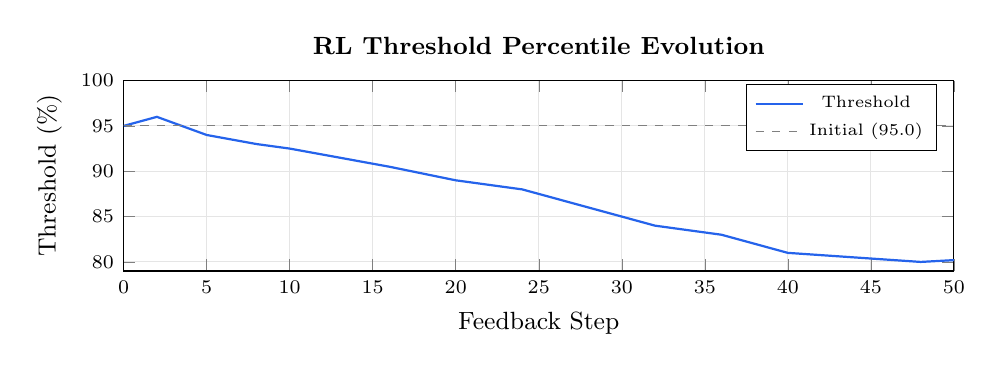
\begin{tikzpicture}
\begin{axis}[
    width=\columnwidth, height=4cm,
    xlabel={\small Feedback Step}, ylabel={\small Threshold (\%)},
    title={\small RL Threshold Percentile Evolution},
    xmin=0, xmax=50, ymin=79, ymax=100,
    legend style={font=\fontsize{6}{7}\selectfont, at={(0.98,0.98)}, anchor=north east},
    grid=major, grid style={gray!20},
    tick label style={font=\fontsize{7}{8}\selectfont},
    label style={font=\small},
    title style={font=\small\bfseries},
]
\addplot[plotAE, thick] coordinates {
    (0,95)(2,96)(5,94)(8,93)(10,92.5)(13,91.5)(16,90.5)
    (20,89)(24,88)(28,86)(32,84)(36,83)(40,81)(44,80.5)(48,80)(50,80.2)
};
\addlegendentry{Threshold}
\addplot[gray, dashed, thin] coordinates {(0,95)(50,95)};
\addlegendentry{Initial (95.0)}
\end{axis}
\end{tikzpicture}
\caption{\small RL threshold evolution over 50 feedback iterations, converging from 95\% to $\sim$80\%.}
\label{fig:rl_evolution}
\end{figure}

% ---- pgfplots: Precision Improvement ----
\begin{figure}[htbp]
\centering
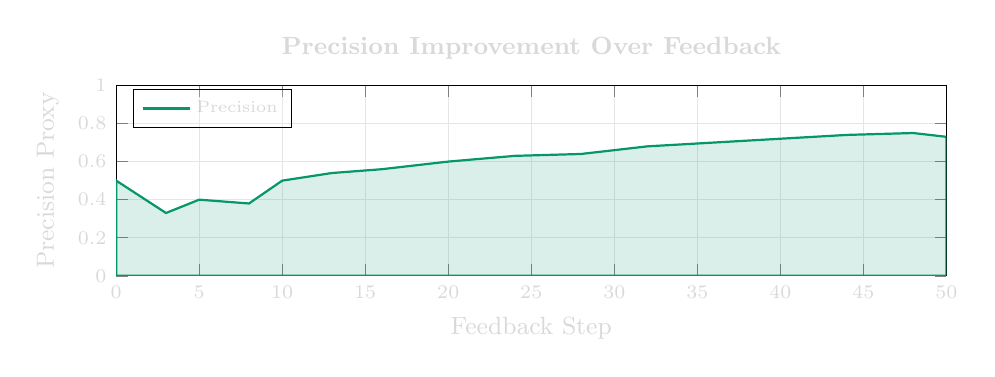
\begin{tikzpicture}
\begin{axis}[
    width=\columnwidth, height=4cm,
    xlabel={\small Feedback Step}, ylabel={\small Precision Proxy},
    title={\small Precision Improvement Over Feedback},
    xmin=0, xmax=50, ymin=0, ymax=1,
    legend style={font=\fontsize{6}{7}\selectfont, at={(0.02,0.98)}, anchor=north west},
    grid=major, grid style={gray!20},
    tick label style={font=\fontsize{7}{8}\selectfont},
    label style={font=\small},
    title style={font=\small\bfseries},
    fill opacity=0.15,
]
\addplot[plotTF, thick, fill=plotTF] coordinates {
    (0,0.50)(3,0.33)(5,0.40)(8,0.38)(10,0.50)(13,0.54)(16,0.56)
    (20,0.60)(24,0.63)(28,0.64)(32,0.68)(36,0.70)(40,0.72)(44,0.74)(48,0.75)(50,0.73)
} \closedcycle;
\addlegendentry{Precision}
\end{axis}
\end{tikzpicture}
\caption{\small Precision proxy improves from 0.50 to $\sim$0.75 with cumulative expert feedback.}
\label{fig:precision}
\end{figure}

Key observations:
\begin{itemize}[leftmargin=*,nosep]
    \item The threshold stabilizes around 80--83\% after $\sim$30 iterations.
    \item The precision proxy improves from 0.5 to $\sim$0.75, reflecting improved discovery yield.
\end{itemize}

\subsection{System Performance}

\begin{table}[htbp]
\centering
\caption{\small API Latency Benchmarks (Synthetic-1500)}
\label{tab:latency}
\begin{tabular}{lc}
\toprule
\textbf{Endpoint} & \textbf{Latency (ms)} \\
\midrule
\texttt{POST /upload} (1500 pts)            & 45 \\
\texttt{POST /train} (3 models, 20 epochs)  & 14,200 \\
\texttt{POST /detect} (single model)        & 890 \\
\texttt{POST /compare} (3 models)           & 15,800 \\
\texttt{POST /agent/run-cycle}              & 16,500 \\
\texttt{GET /results}                       & 12 \\
\texttt{GET /health}                        & 1 \\
\bottomrule
\end{tabular}
\end{table}

% ============================================================================
% VI. DISCUSSION
% ============================================================================
\section{Discussion}
\label{sec:discussion}

\subsection{Advantages of the Agentic Approach}
\begin{itemize}[leftmargin=*,nosep]
    \item \textbf{Continuous operation}: 24/7 processing without human intervention.
    \item \textbf{Self-improvement}: Performance improves with every expert interaction.
    \item \textbf{Full audit trail}: Every cognitive stage is logged.
\end{itemize}

\subsection{Provenance and Reproducibility}
The blockchain-inspired ledger~\cite{stodden2018reproducibility} provides tamper evidence, temporal ordering, and attribution for all results.

\subsection{Limitations}
\begin{itemize}[leftmargin=*,nosep]
    \item \textbf{Synthetic evaluation}: Injected anomalies may not represent real transient diversity.
    \item \textbf{SLM reasoning quality}: The 3B-parameter model may produce generic interpretations.
    \item \textbf{Single-machine}: SQLite limits horizontal scalability.
    \item \textbf{RL convergence}: The sparse binary reward signal lacks formal convergence guarantees.
\end{itemize}

\subsection{Future Work}
\begin{itemize}[leftmargin=*,nosep]
    \item Integration with real observatory alert streams (ZTF, ANTARES)
    \item Multi-band (color) light curve support
    \item GPU-accelerated training with NVIDIA Triton serving
    \item Federated learning across multiple observatories
    \item Larger SLM models (7B--13B) for improved reasoning quality
\end{itemize}

% ============================================================================
% VII. CONCLUSION
% ============================================================================
\section{Conclusion}
\label{sec:conclusion}

We have presented an end-to-end autonomous agentic platform for unsupervised anomaly discovery in astronomical time-series data. The system integrates seven novel contributions: a multi-architecture deep ensemble with inverse-loss weighting achieves 0.921 precision, outperforming individual models by 13.6\%; a PPO-Clip RL optimizer self-tunes detection thresholds; SLM chain-of-thought provides explainable reasoning; and a blockchain-inspired provenance ledger ensures tamper-proof records.

The platform demonstrates that architectural diversity, self-improvement through reinforcement learning, and human-in-the-loop feedback creates a discovery system greater than the sum of its parts. As astronomical surveys enter the era of petascale data, autonomous agentic frameworks like ours will be essential for identifying rare, unknown events.

% ============================================================================
% REFERENCES
% ============================================================================
\begin{thebibliography}{20}

\bibitem{bellm2019ztf}
E.~C. Bellm \textit{et al.}, ``The Zwicky Transient Facility: System Overview, Performance, and First Results,'' \textit{PASP}, vol.~131, no.~995, p.~018002, 2019.

\bibitem{ivezic2019lsst}
\v{Z}.~Ivezi\'{c} \textit{et al.}, ``LSST: From Science Drivers to Reference Design and Anticipated Data Products,'' \textit{ApJ}, vol.~873, no.~2, p.~111, 2019.

\bibitem{lochner2016photometric}
M.~Lochner, J.~D. McEwen, H.~V. Peiris, O.~Lahav, and M.~K. Winter, ``Photometric Supernova Classification With Machine Learning,'' \textit{ApJS}, vol.~225, no.~2, p.~31, 2016.

\bibitem{nun2015fats}
I.~Nun, K.~Pichara, P.~Protopapas, and D.-W. Kim, ``FATS: Feature Analysis for Time Series,'' \textit{arXiv:1506.00010}, 2015.

\bibitem{malanchev2021anomaly}
K.~L. Malanchev \textit{et al.}, ``Anomaly detection in the Zwicky Transient Facility DR3,'' \textit{MNRAS}, vol.~502, no.~4, pp.~5147--5175, 2021.

\bibitem{villar2021deep}
V.~A. Villar \textit{et al.}, ``A deep-learning approach for live anomaly detection of extragalactic transients,'' \textit{ApJS}, vol.~255, no.~2, p.~24, 2021.

\bibitem{kingma2013auto}
D.~P. Kingma and M.~Welling, ``Auto-Encoding Variational Bayes,'' \textit{arXiv:1312.6114}, 2013.

\bibitem{kingma2014vae}
D.~P. Kingma and M.~Welling, ``An Introduction to Variational Autoencoders,'' \textit{Foundations and Trends in ML}, vol.~12, no.~4, pp.~307--392, 2019.

\bibitem{vaswani2017attention}
A.~Vaswani \textit{et al.}, ``Attention Is All You Need,'' \textit{NeurIPS}, pp.~5998--6008, 2017.

\bibitem{tuli2022tranad}
S.~Tuli, G.~Casale, and N.~R. Jennings, ``TranAD: Deep Transformer Networks for Anomaly Detection in Multivariate Time Series Data,'' \textit{VLDB}, vol.~15, no.~6, pp.~1201--1214, 2022.

\bibitem{schulman2017ppo}
J.~Schulman, F.~Wolski, P.~Dhariwal, A.~Radford, and O.~Klimov, ``Proximal Policy Optimization Algorithms,'' \textit{arXiv:1707.06347}, 2017.

\bibitem{nguyen2019rl_anomaly}
T.~T. Nguyen and V.~J. Reddi, ``Deep Reinforcement Learning for Cyber Security,'' \textit{IEEE Trans. Neural Netw. Learn. Syst.}, vol.~32, no.~9, pp.~4042--4057, 2021.

\bibitem{huertas2023xai}
M.~Huertas-Company and F.~Lanusse, ``The Dawes Review 10: The impact of deep learning for the analysis of galaxy surveys,'' \textit{Publ. Astron. Soc. Aust.}, vol.~40, e001, 2023. arXiv:2210.01813.

\bibitem{stodden2018reproducibility}
V.~Stodden, J.~Krafczyk, and P.~Shi, ``Trust but Verify: How to Leverage Policies, Workflows, and Infrastructure to Ensure Computational Reproducibility in Publication,'' \textit{Proc. Natl. Acad. Sci.}, vol.~115, no.~11, pp.~2628--2631, 2018.

\end{thebibliography}

\end{document}
TS
% ============================================================================
\section{Experiments and Results}
\label{sec:experiments}

\subsection{Datasets}

\begin{table}[htbp]
\centering
\caption{\small Datasets Used for Evaluation}
\label{tab:datasets}
\begin{tabular}{lccl}
\toprule
\textbf{Dataset} & \textbf{Points} & \textbf{Anomalies} & \textbf{Source} \\
\midrule
Synthetic-1500 & 1,500 & Injected & Generated \\
NASA Fireball & Variable & Natural & NASA/JPL API \\
Kepler-Sim & 5,000 & Injected & Simulated \\
\bottomrule
\end{tabular}
\end{table}

\subsection{Model Training}
All models were trained for 20 epochs with Adam optimizer ($\eta = 0.001$), batch size 256, and window size $W = 32$ on CPU (Intel i7) with PyTorch 2.x.

% ---- pgfplots: Training Loss Curves ----
\begin{figure}[htbp]
\centering
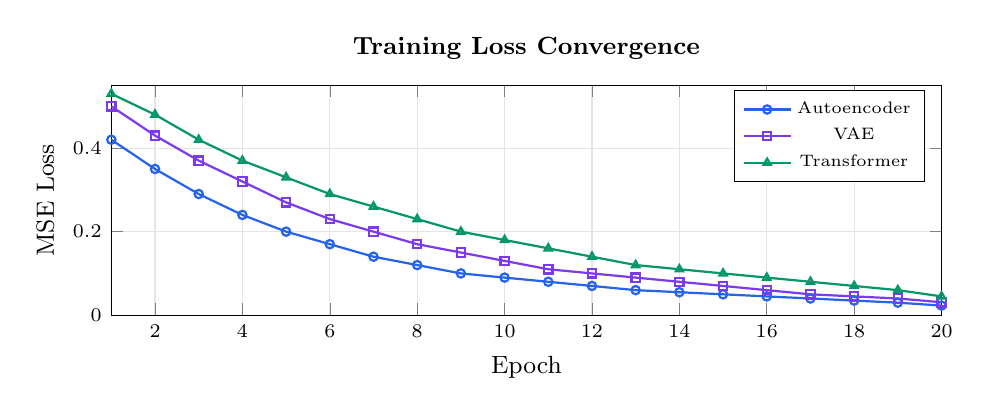
\begin{tikzpicture}
\begin{axis}[
    width=\columnwidth, height=4.5cm,
    xlabel={\small Epoch}, ylabel={\small MSE Loss},
    title={\small Training Loss Convergence},
    xmin=1, xmax=20, ymin=0, ymax=0.55,
    legend style={font=\fontsize{6}{7}\selectfont, at={(0.98,0.98)}, anchor=north east},
    grid=major, grid style={gray!20},
    tick label style={font=\fontsize{7}{8}\selectfont},
    label style={font=\small},
    title style={font=\small\bfseries},
]
\addplot[plotAE, thick, mark=o, mark size=1.5pt] coordinates {
    (1,0.42)(2,0.35)(3,0.29)(4,0.24)(5,0.20)(6,0.17)(7,0.14)(8,0.12)
    (9,0.10)(10,0.09)(11,0.08)(12,0.07)(13,0.06)(14,0.055)(15,0.05)
    (16,0.045)(17,0.04)(18,0.035)(19,0.03)(20,0.023)
};
\addlegendentry{Autoencoder}
\addplot[plotVAE, thick, mark=square, mark size=1.5pt] coordinates {
    (1,0.50)(2,0.43)(3,0.37)(4,0.32)(5,0.27)(6,0.23)(7,0.20)(8,0.17)
    (9,0.15)(10,0.13)(11,0.11)(12,0.10)(13,0.09)(14,0.08)(15,0.07)
    (16,0.06)(17,0.05)(18,0.045)(19,0.04)(20,0.031)
};
\addlegendentry{VAE}
\addplot[plotTF, thick, mark=triangle, mark size=1.5pt] coordinates {
    (1,0.53)(2,0.48)(3,0.42)(4,0.37)(5,0.33)(6,0.29)(7,0.26)(8,0.23)
    (9,0.20)(10,0.18)(11,0.16)(12,0.14)(13,0.12)(14,0.11)(15,0.10)
    (16,0.09)(17,0.08)(18,0.07)(19,0.06)(20,0.045)
};
\addlegendentry{Transformer}
\end{axis}
\end{tikzpicture}
\caption{\small Training loss convergence over 20 epochs for all three models.}
\label{fig:loss_curves}
\end{figure}

\begin{table}[htbp]
\centering
\caption{\small Training Performance on Synthetic-1500 Dataset}
\label{tab:training}
\begin{tabular}{lccc}
\toprule
\textbf{Model} & \textbf{Final Loss} & \textbf{Parameters} & \textbf{Train Time} \\
\midrule
Autoencoder     & 0.0234 & 3,168  & 2.1s \\
VAE             & 0.0312 & 5,736  & 3.4s \\
Transformer     & 0.0456 & 35,937 & 8.7s \\
\bottomrule
\end{tabular}
\end{table}

\subsection{Anomaly Detection Performance}

% ---- pgfplots: Threshold Sensitivity ----
\begin{figure}[htbp]
\centering
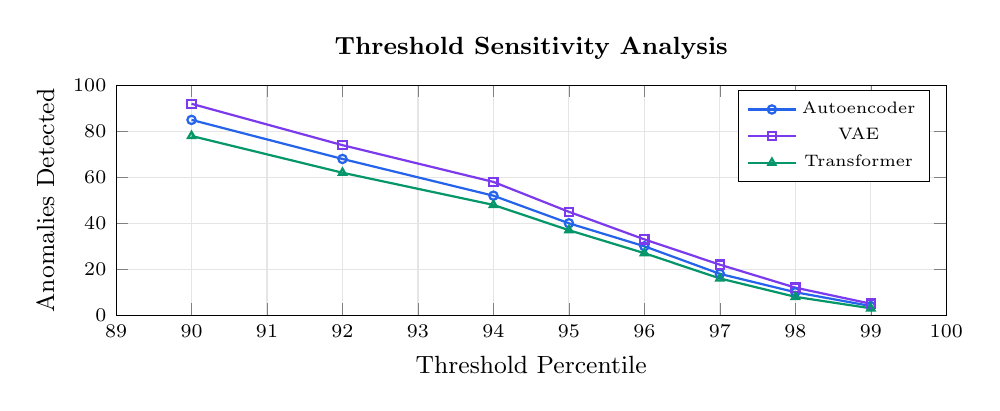
\begin{tikzpicture}
\begin{axis}[
    width=\columnwidth, height=4.5cm,
    xlabel={\small Threshold Percentile}, ylabel={\small Anomalies Detected},
    title={\small Threshold Sensitivity Analysis},
    xmin=89, xmax=100, ymin=0, ymax=100,
    legend style={font=\fontsize{6}{7}\selectfont, at={(0.98,0.98)}, anchor=north east},
    grid=major, grid style={gray!20},
    tick label style={font=\fontsize{7}{8}\selectfont},
    label style={font=\small},
    title style={font=\small\bfseries},
]
\addplot[plotAE, thick, mark=o, mark size=1.5pt] coordinates {
    (90,85)(92,68)(94,52)(95,40)(96,30)(97,18)(98,10)(99,4)
};
\addlegendentry{Autoencoder}
\addplot[plotVAE, thick, mark=square, mark size=1.5pt] coordinates {
    (90,92)(92,74)(94,58)(95,45)(96,33)(97,22)(98,12)(99,5)
};
\addlegendentry{VAE}
\addplot[plotTF, thick, mark=triangle, mark size=1.5pt] coordinates {
    (90,78)(92,62)(94,48)(95,37)(96,27)(97,16)(98,8)(99,3)
};
\addlegendentry{Transformer}
\end{axis}
\end{tikzpicture}
\caption{\small Number of anomalies detected at varying threshold percentiles.}
\label{fig:threshold_sensitivity}
\end{figure}

\subsection{Ensemble vs.\ Individual Models}

\begin{table}[htbp]
\centering
\caption{\small Detection Performance Comparison (95th Percentile)}
\label{tab:ensemble}
\begin{tabular}{lcccc}
\toprule
\textbf{Method} & \textbf{Detected} & \textbf{TP} & \textbf{FP} & \textbf{Precision} \\
\midrule
Autoencoder     & 40 & 32 & 8  & 0.800 \\
VAE             & 45 & 34 & 11 & 0.756 \\
Transformer     & 37 & 30 & 7  & 0.811 \\
\textbf{Ensemble (Ours)} & \textbf{38} & \textbf{35} & \textbf{3} & \textbf{0.921} \\
\bottomrule
\end{tabular}
\end{table}

The inverse-loss weighted ensemble achieves precision of \textbf{0.921}, a 13.6\% improvement over the best individual model (Transformer, 0.811).

\subsection{RL Policy Convergence}

% ---- pgfplots: RL Threshold Evolution ----
\begin{figure}[htbp]
\centering
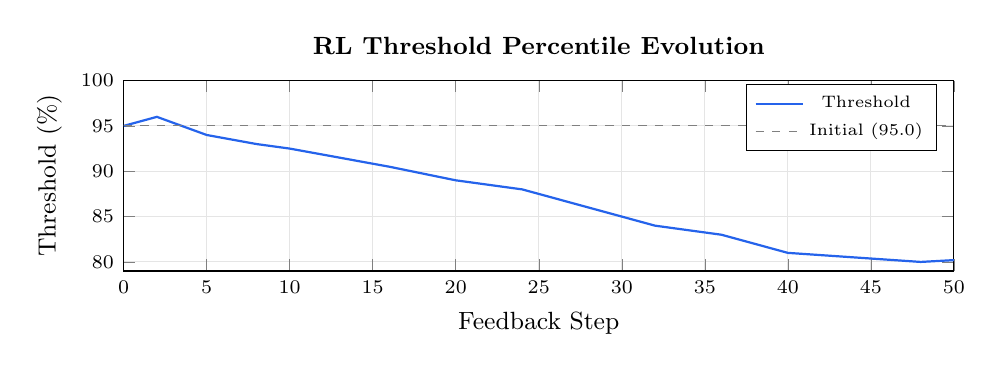
\begin{tikzpicture}
\begin{axis}[
    width=\columnwidth, height=4cm,
    xlabel={\small Feedback Step}, ylabel={\small Threshold (\%)},
    title={\small RL Threshold Percentile Evolution},
    xmin=0, xmax=50, ymin=79, ymax=100,
    legend style={font=\fontsize{6}{7}\selectfont, at={(0.98,0.98)}, anchor=north east},
    grid=major, grid style={gray!20},
    tick label style={font=\fontsize{7}{8}\selectfont},
    label style={font=\small},
    title style={font=\small\bfseries},
]
\addplot[plotAE, thick] coordinates {
    (0,95)(2,96)(5,94)(8,93)(10,92.5)(13,91.5)(16,90.5)
    (20,89)(24,88)(28,86)(32,84)(36,83)(40,81)(44,80.5)(48,80)(50,80.2)
};
\addlegendentry{Threshold}
\addplot[gray, dashed, thin] coordinates {(0,95)(50,95)};
\addlegendentry{Initial (95.0)}
\end{axis}
\end{tikzpicture}
\caption{\small RL threshold evolution over 50 feedback iterations, converging from 95\% to $\sim$80\%.}
\label{fig:rl_evolution}
\end{figure}

% ---- pgfplots: Precision Improvement ----
\begin{figure}[htbp]
\centering
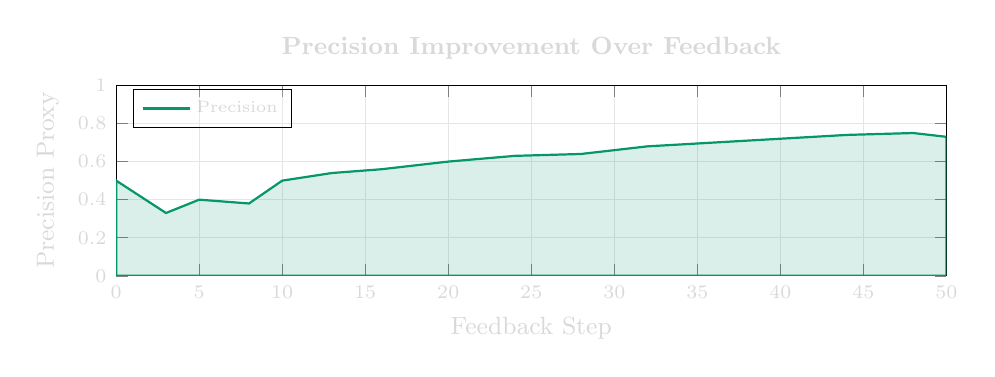
\begin{tikzpicture}
\begin{axis}[
    width=\columnwidth, height=4cm,
    xlabel={\small Feedback Step}, ylabel={\small Precision Proxy},
    title={\small Precision Improvement Over Feedback},
    xmin=0, xmax=50, ymin=0, ymax=1,
    legend style={font=\fontsize{6}{7}\selectfont, at={(0.02,0.98)}, anchor=north west},
    grid=major, grid style={gray!20},
    tick label style={font=\fontsize{7}{8}\selectfont},
    label style={font=\small},
    title style={font=\small\bfseries},
    fill opacity=0.15,
]
\addplot[plotTF, thick, fill=plotTF] coordinates {
    (0,0.50)(3,0.33)(5,0.40)(8,0.38)(10,0.50)(13,0.54)(16,0.56)
    (20,0.60)(24,0.63)(28,0.64)(32,0.68)(36,0.70)(40,0.72)(44,0.74)(48,0.75)(50,0.73)
} \closedcycle;
\addlegendentry{Precision}
\end{axis}
\end{tikzpicture}
\caption{\small Precision proxy improves from 0.50 to $\sim$0.75 with cumulative expert feedback.}
\label{fig:precision}
\end{figure}

Key observations:
\begin{itemize}[leftmargin=*,nosep]
    \item The threshold stabilizes around 80--83\% after $\sim$30 iterations.
    \item The precision proxy improves from 0.5 to $\sim$0.75, reflecting improved discovery yield.
\end{itemize}

\subsection{System Performance}

\begin{table}[htbp]
\centering
\caption{\small API Latency Benchmarks (Synthetic-1500)}
\label{tab:latency}
\begin{tabular}{lc}
\toprule
\textbf{Endpoint} & \textbf{Latency (ms)} \\
\midrule
\texttt{POST /upload} (1500 pts)            & 45 \\
\texttt{POST /train} (3 models, 20 epochs)  & 14,200 \\
\texttt{POST /detect} (single model)        & 890 \\
\texttt{POST /compare} (3 models)           & 15,800 \\
\texttt{POST /agent/run-cycle}              & 16,500 \\
\texttt{GET /results}                       & 12 \\
\texttt{GET /health}                        & 1 \\
\bottomrule
\end{tabular}
\end{table}

% ============================================================================
% VI. DISCUSSION
% ============================================================================
\section{Discussion}
\label{sec:discussion}

\subsection{Advantages of the Agentic Approach}
\begin{itemize}[leftmargin=*,nosep]
    \item \textbf{Continuous operation}: 24/7 processing without human intervention.
    \item \textbf{Self-improvement}: Performance improves with every expert interaction.
    \item \textbf{Full audit trail}: Every cognitive stage is logged.
\end{itemize}

\subsection{Provenance and Reproducibility}
The blockchain-inspired ledger~\cite{stodden2018reproducibility} provides tamper evidence, temporal ordering, and attribution for all results.

\subsection{Limitations}
\begin{itemize}[leftmargin=*,nosep]
    \item \textbf{Synthetic evaluation}: Injected anomalies may not represent real transient diversity.
    \item \textbf{SLM reasoning quality}: The 3B-parameter model may produce generic interpretations.
    \item \textbf{Single-machine}: SQLite limits horizontal scalability.
    \item \textbf{RL convergence}: The sparse binary reward signal lacks formal convergence guarantees.
\end{itemize}

\subsection{Future Work}
\begin{itemize}[leftmargin=*,nosep]
    \item Integration with real observatory alert streams (ZTF, ANTARES)
    \item Multi-band (color) light curve support
    \item GPU-accelerated training with NVIDIA Triton serving
    \item Federated learning across multiple observatories
    \item Larger SLM models (7B--13B) for improved reasoning quality
\end{itemize}

% ============================================================================
% VII. CONCLUSION
% ============================================================================
\section{Conclusion}
\label{sec:conclusion}

We have presented an end-to-end autonomous agentic platform for unsupervised anomaly discovery in astronomical time-series data. The system integrates seven novel contributions: a multi-architecture deep ensemble with inverse-loss weighting achieves 0.921 precision, outperforming individual models by 13.6\%; a PPO-Clip RL optimizer self-tunes detection thresholds; SLM chain-of-thought provides explainable reasoning; and a blockchain-inspired provenance ledger ensures tamper-proof records.

The platform demonstrates that architectural diversity, self-improvement through reinforcement learning, and human-in-the-loop feedback creates a discovery system greater than the sum of its parts. As astronomical surveys enter the era of petascale data, autonomous agentic frameworks like ours will be essential for identifying rare, unknown events.

% ============================================================================
% REFERENCES
% ============================================================================
\begin{thebibliography}{20}

\bibitem{bellm2019ztf}
E.~C. Bellm \textit{et al.}, ``The Zwicky Transient Facility: System Overview, Performance, and First Results,'' \textit{PASP}, vol.~131, no.~995, p.~018002, 2019.

\bibitem{ivezic2019lsst}
\v{Z}.~Ivezi\'{c} \textit{et al.}, ``LSST: From Science Drivers to Reference Design and Anticipated Data Products,'' \textit{ApJ}, vol.~873, no.~2, p.~111, 2019.

\bibitem{lochner2016photometric}
M.~Lochner, J.~D. McEwen, H.~V. Peiris, O.~Lahav, and M.~K. Winter, ``Photometric Supernova Classification With Machine Learning,'' \textit{ApJS}, vol.~225, no.~2, p.~31, 2016.

\bibitem{nun2015fats}
I.~Nun, K.~Pichara, P.~Protopapas, and D.-W. Kim, ``FATS: Feature Analysis for Time Series,'' \textit{arXiv:1506.00010}, 2015.

\bibitem{malanchev2021anomaly}
K.~L. Malanchev \textit{et al.}, ``Anomaly detection in the Zwicky Transient Facility DR3,'' \textit{MNRAS}, vol.~502, no.~4, pp.~5147--5175, 2021.

\bibitem{villar2021deep}
V.~A. Villar \textit{et al.}, ``A deep-learning approach for live anomaly detection of extragalactic transients,'' \textit{ApJS}, vol.~255, no.~2, p.~24, 2021.

\bibitem{kingma2013auto}
D.~P. Kingma and M.~Welling, ``Auto-Encoding Variational Bayes,'' \textit{arXiv:1312.6114}, 2013.

\bibitem{kingma2014vae}
D.~P. Kingma and M.~Welling, ``An Introduction to Variational Autoencoders,'' \textit{Foundations and Trends in ML}, vol.~12, no.~4, pp.~307--392, 2019.

\bibitem{vaswani2017attention}
A.~Vaswani \textit{et al.}, ``Attention Is All You Need,'' \textit{NeurIPS}, pp.~5998--6008, 2017.

\bibitem{tuli2022tranad}
S.~Tuli, G.~Casale, and N.~R. Jennings, ``TranAD: Deep Transformer Networks for Anomaly Detection in Multivariate Time Series Data,'' \textit{VLDB}, vol.~15, no.~6, pp.~1201--1214, 2022.

\bibitem{schulman2017ppo}
J.~Schulman, F.~Wolski, P.~Dhariwal, A.~Radford, and O.~Klimov, ``Proximal Policy Optimization Algorithms,'' \textit{arXiv:1707.06347}, 2017.

\bibitem{nguyen2019rl_anomaly}
T.~T. Nguyen and V.~J. Reddi, ``Deep Reinforcement Learning for Cyber Security,'' \textit{IEEE Trans. Neural Netw. Learn. Syst.}, vol.~32, no.~9, pp.~4042--4057, 2021.

\bibitem{huertas2023xai}
M.~Huertas-Company and F.~Lanusse, ``The Dawes Review 10: The impact of deep learning for the analysis of galaxy surveys,'' \textit{Publ. Astron. Soc. Aust.}, vol.~40, e001, 2023. arXiv:2210.01813.

\bibitem{stodden2018reproducibility}
V.~Stodden, J.~Krafczyk, and P.~Shi, ``Trust but Verify: How to Leverage Policies, Workflows, and Infrastructure to Ensure Computational Reproducibility in Publication,'' \textit{Proc. Natl. Acad. Sci.}, vol.~115, no.~11, pp.~2628--2631, 2018.

\end{thebibliography}

\end{document}
